\documentclass[12pt,letterpaper,oneside,reqno]{amsart}
\usepackage{amsfonts}
\usepackage{amsmath}
\usepackage{amssymb}
\usepackage{amsthm}
\usepackage{float}
\usepackage{mathrsfs}
\usepackage{colonequals}
\usepackage[font=small,labelfont=bf]{caption}
\usepackage[unicode,pdfpagelabels,hyperindex,colorlinks=true,linkcolor=blue,urlcolor=blue,citecolor=blue]{hyperref}
\usepackage{graphicx}
\emergencystretch=1em
\usepackage{array}
\usepackage{enumitem}
\usepackage{etoolbox}
\usepackage{physics}
\usepackage{booktabs}

% margins and layout
\linespread{1.7}
\usepackage[left=1in,right=1in,bottom=1in,top=1in]{geometry}
\apptocmd{\sloppy}{\hbadness 10000\relax}{}{}
\raggedbottom

\newcommand \coeffA [3][A] {{\mathbf{#1}} \sb{#2,#3}}
\newcommand \polynomialP [4][P]{{\mathbf{#1}}\sp{#2} \sb{#3}(#4)}
\newcommand \bernoulli [2][B] {{#1}\sb{#2}}


\newtheorem{theorem}{Theorem}[section]
\newtheorem{corollary}[theorem]{Corollary}
\newtheorem{proposition}[theorem]{Proposition}
\newtheorem{observation}[theorem]{Observation}
\newtheorem{lemma}[theorem]{Lemma}
\newtheorem{claim}[theorem]{Claim}
\newtheorem{example}[theorem]{Example}
\newtheorem{conjecture}[theorem]{Conjecture}
\newtheorem{definition}[theorem]{Definition}
\newtheorem{question}[theorem]{Question}
\newtheorem{remark}[theorem]{Remark}
\newtheorem{assumption}[theorem]{Assumption}

%\numberwithin{equation}{section}

\title[Unexpected polynomial identities arising from a class. interpolation problem]
{Unexpected polynomial identities arising from a classical interpolation problem}
\author[Petro Kolosov]{Petro Kolosov}
\date{\today}

% metadata
\email{kolosovp94@gmail.com}
\address{Software Developer, DevOps Engineer}
\urladdr{https://kolosovpetro.github.io}
\subjclass[2010]{05A19, 05A10, 41A15, 11B83, 68W30}
\keywords{Polynomial identities,
    Finite differences,
    Binomial coefficients,
    Faulhaber's formula,
    Sums of powers,
    Bernoulli numbers,
    Combinatorics,
    Pascal's triangle,
    OEIS}
\hypersetup{
    pdftitle={Unexpected Polynomial Identities arising from a Classical Interpolation Problem},
    pdfproducer={LaTeX},
    pdfcreator={pdflatex},
    pdfauthor={Petro Kolosov},
    pdfsubject={New Polynomial Identities that motivated by Classical Interpolation Problem},
    pdfkeywords={Polynomial identities,
    Finite differences,
    Binomial coefficients,
    Faulhaber's formula,
    Sums of powers,
    Power sums,
    Bernoulli numbers,
    Combinatorics,
    Pascal's triangle,
    OEIS}
}

\begin{document}

    \begin{abstract}
        This manuscript originates from a classical interpolation problem: how to reconstruct the cubes $n^3$
from their finite differences.
The investigation leads to an unexpected identity expressing $n^3$ as sum of bivariate terms $k(n-k)$,
such that $n^3=\sum_{k=1}^{n} 6k(n-k) + 1$.
This identity serves as the base case for a more general identity for odd powers,
involving rational numbers $\mathbf{A}_{m,r}$ that is
$n^{2m+1} = \sum_{k=1}^{n} \sum_{r=0}^{m} \mathbf{A}_{m,r} k^r (n-k)^r$.
We evaluate the set of coefficients $\mathbf{A}_{m,0}, \mathbf{A}_{m,1}, \cdots, \mathbf{A}_{m,m}$
by solving a system of linear equations.
Furthermore, this work provides a recurrence relation
for coefficients $\mathbf{A}_{m,0}, \mathbf{A}_{m,1}, \cdots, \mathbf{A}_{m,m}$, by utilizing
generating functions.
The main results include odd power identities, identities for binomial forms,
and identities for sums of powers.
Apart that, we discuss the similarities between our findings and well-known results like Pascal's identity etc.
Afterward, the manuscript continues with related works that are based on our findings,
including approximation for powers,
derivatives, Faulhaber-like formulas.
This manuscript concludes with discussion of future research directions that include
the topics of integration into mathematical literature, approximation methods, combinatorial interpretations,
and $q$-Derivatives.

    \end{abstract}

    \maketitle

    \tableofcontents


    \section{Discussion on interpolation of cubes}
    \label{sec:the-problem-of-interpolation-of-cubes}
    This is the story of a student with a deep curiosity for mathematics.
Although, not a specialist in mathematics,
our young explorer always possessed a strong sense of mathematical beauty and aesthetics.
The mathematical knowledge of the individual was limited by undergraduate level course, which includes the basics of
matrix operations, basic calculus, and elementary linear algebra.
One day, our student found himself observing the tables of finite differences, precisely finite differences of cubes.

By observing the table
\begin{table}[H]
    \begin{center}
        \setlength\extrarowheight{-6pt}
        \begin{tabular}{c|cccc}
            $n$ & $n^3$ & $\Delta(n^3)$ & $\Delta^2(n^3)$ & $\Delta^3(n^3)$ \\
            \hline
            0   & 0     & 1             & 6               & 6               \\
            1   & 1     & 7             & 12              & 6               \\
            2   & 8     & 19            & 18              & 6               \\
            3   & 27    & 37            & 24              & 6               \\
            4   & 64    & 61            & 30              & 6               \\
            5   & 125   & 91            & 36              &                 \\
            6   & 216   & 127           &                 &                 \\
            7   & 343   &               &                 &
        \end{tabular}
    \end{center}
    \caption{Table of finite differences of the polynomial $n^3$.} \label{tab:table}
\end{table}

The first question that visited curious mind was
\begin{question}
    \label{quest:interpolation-cubes}
    How to reconstruct the value of $n^3$ from the values of its finite differences?
\end{question}
Precisely, the inquiry is to find a way to reconstruct the values of the sequence $\{0, 1, 8, 27, 64, \ldots\}$
given the values of finite differences in the table~\eqref{tab:finite-differences-cubes}.

In its essence, the problem is so old that it can be traced back
to ancient Babylonian and Greek times, several centuries BC and first centuries AD~\cite{gautschi2012interpolation}.
The process of finding new data points based on the range of a discrete set
of known data points is called interpolation.
Interpolation, as we know it today, was developed in 1674--1684 by Isaac Newton
in his works referenced as foundation of classical interpolation theory~\cite{meijering2002chronology}.
For instance, Newton's interpolation formula addresses the question~\eqref{quest:interpolation-cubes} immediately,
because
\begin{align*}
    27 = 6 \binom{3}{3} + 6 \binom{3}{2} + 1 \binom{3}{1} + 0\binom{3}{0} = 6 + 18 + 3
\end{align*}
where $6,6,1,0$ is the first row in table~\eqref{tab:finite-differences-cubes}.
In general,
\begin{align*}
    n^3 = 6 \binom{n}{3} + 6 \binom{n}{2} + 1\binom{n}{1} + 0 \binom{n}{0}
\end{align*}
because $f(x) = \sum_{k=0}^{d} \Delta^{d-k} f(0) \binom{x}{d-k}$, see~\cite[~p. 190]{graham1994concrete}.

Great!
But there is one thing, the student who has risen the question~\eqref{quest:interpolation-cubes}
had no clue about interpolation theory at all.
What was decided then?
Exactly, our inquirer has decided to find a solution himself, being driven by the pure feeling of mystery.
His mind was occupied by only a single thought:
\textit{All mathematical truths exist timelessly, we only reveal and describe them.}
That mindset inspired our student to start his own mathematical journey.

By observing the table of finite differences~\eqref{tab:finite-differences-cubes} we can notice that
the first finite difference of cubes may be expressed in terms of its
third finite differences $\Delta^3(n^3) = 6$, as follows
\begin{align*}
    \begin{split}
        \Delta(0^3) &= 1+6 \cdot 0 \\
        \Delta(1^3) &= 1+6\cdot0+6\cdot1 \\
        \Delta(2^3) &= 1+6\cdot0+6\cdot1+6\cdot2 \\
        \Delta(3^3) &= 1+6\cdot0+6\cdot1+6\cdot2+6\cdot3 \\
        &\; \; \vdots \\
        \Delta(n^3) &= 1+6\cdot0+6\cdot1+6\cdot2+6\cdot3 + \cdots + 6n
    \end{split}
\end{align*}
By using sigma notation, we get
\begin{align*}
    \Delta(n^3) = 1+6\cdot0+6\cdot1+6\cdot2+6\cdot3+\cdots+6\cdot n = 1 + 6 \sum_{k=0}^{n} k
\end{align*}

However, there is a more beautiful way to prove that $\Delta(n^3) = 1 + 6 \sum_{k=0}^{n} k$.
We refer to one of the finest articles in the area of polynomials and power sums,
that is \textit{Johann Faulhaber and sums of powers} written by Donald Knuth~\cite{knuth1993johann}.
Indeed, this article is a great mean to reach piece of mind in mathematics.
We now focus on the odd power identities shown at~\cite[~p. 9]{knuth1993johann}
\begin{align*}
    n^1 &= \binom{n}{1} \\
    n^3 &= 6 \binom{n+1}{3} + \binom{n}{1} \\
    n^5 &= 120 \binom{n+2}{5} + 30 \binom{n+1}{3} + \binom{n}{1}
\end{align*}

It is quite interesting that the identity in terms of triangular numbers $\binom{n+1}{2}$
and finite differences of cubes becomes more obvious
\begin{align*}
    \Delta n^3
    = (n+1)^3 - n^3
    =  6 \binom{n+1}{2} + \binom{n}{0}
\end{align*}
It easy to see that
\begin{align*}
    \Delta n^3
    = \left[ 6 \binom{n+2}{3} + \binom{n+1}{1} \right] - \left[ 6 \binom{n+1}{3} + \binom{n}{1} \right]
    = 6 \binom{n+1}{2} + \binom{n}{0}
\end{align*}
because $\binom{n}{k} = \binom{n-1}{k} + \binom{n-1}{k-1}$.

Moreover, the concept above allows us to reach $N$-fold power sums $\sum^N k^{2m+1}$
or finite differences $\Delta^N k^{2m+1}$ by simply altering
binomial coefficients indexes.
Quite strong and impressive.

We can observe that triangular numbers $\binom{n+1}{2}$ are equivalent to
\begin{align*}
    \binom{n+1}{2} = \sum_{k=0}^{n} \binom{k}{1} = \sum_{k=0}^{n} k
\end{align*}
because $\binom{n+1}{m+1} = \sum_{k=0}^{n} \binom{k}{m}$.
This leads us to the fact that
\begin{align*}
    \Delta n^3 = (n+1)^3 - n^3 = 1 + 6 \sum_{k=0}^{n} k
\end{align*}
An experienced mathematician would immediately notice a spot to apply Faulhaber's formula~\cite{beardon1996sums}
to get the closed form of the sum $\sum_{k=0}^{n} k$
\begin{align*}
    \sum_{k=0}^{n} k = \frac{1}{2}(n+n^2)
\end{align*}
Thus, the finite difference $\Delta(n^3)$ takes the well-known form,
which matches Binomial theorem~\cite{abramowitz1988handbook}
\begin{align*}
    \Delta(n^3)
    = 1 + 6 \left[ \frac{1}{2}(n+n^2) \right]
    = 1 + 3 n + 3 n^2
    = \sum_{k=0}^{2} \binom{3}{k} n^k
\end{align*}
And\ldots that could be the end of the story, isn't it?
Because all what remains is to say that
\begin{align*}
    n^3
    = \sum_{k=0}^{n-1} (k+1)^3 - k^3
    = \sum_{k=0}^{n-1} \left( 1 + 6 \sum_{t=0}^{k} t \right)
    = \sum_{k=0}^{n-1} 1 + 3 k + 3 k^2
\end{align*}
Thus, the formula for polynomial $n^3$ is derived successfully, and thus,
our protégée's question~\eqref{quest:interpolation-cubes} is answered positively.
Because we have successfully found the function that matches $n^3$ from the values of its finite differences from the
table~\eqref{tab:finite-differences-cubes}.

However, not this time.
Luckily enough (say), the student who has stated the question~\eqref{quest:interpolation-cubes}
wasn't really aware of the approaches above neither.
What a lazy student!
Probably, that's exactly the case when unawareness leads to a fresh sight to classical questions,
leading to unexpected results and new insights.
Instead, our investigator spotted a little bit different pattern in $\Delta n^3= 6 \binom{n+1}{2} + \binom{n}{0}$.

Consider the polynomial $n^3$ as sum of its finite differences
\begin{align*}
    n^3
    &= [1+6\cdot0] \\
    &+ [1+6\cdot0+6\cdot1] \\
    &+ [1+6\cdot0+6\cdot1+6\cdot2] + \cdots \\
    &+ [1+6\cdot0+6\cdot1+6\cdot2+\cdots+6\cdot(n-1)]
\end{align*}
We can observe that the term $1$ appears $n$ times, the item $6\cdot0$ appears $n-0$ times,
the item $6\cdot1$ appears $n-1$ times and so on.
By rearranging recurring common terms
\begin{align*}
    n^3 = n
    &+ [(n-0) \cdot 6 \cdot 0] \\
    &+ [(n-1)\cdot6\cdot1] \\
    &+ [(n-2)\cdot6\cdot2] + \cdots \\
    &+ [(n-k)\cdot 6 \cdot k] + \cdots \\
    &+ [1\cdot6\cdot(n-1)]
\end{align*}
By applying compact sigma sum notation yields an identity for cubes $n^3$
\begin{align*}
    n^3 = n + \sum_{k=0}^{n-1} 6k(n-k)
\end{align*}
We can freely move the term $n$ under the summation, because there are exactly $n$ iterations.
Therefore,
\begin{align*}
    n^3 = \sum_{k=0}^{n-1} 6k(n-k) + 1
\end{align*}
By inspecting the expression $6k(n-k) + 1$, we can notice that it is symmetric over $k$.
Let be $T_{1} (n,k) = 6k(n-k) + 1$ then
\begin{align*}
    T_{1} (n,k) = T_{1} (n,n-k)
\end{align*}
This symmetry allows us to alter summation bounds easily.
Hence,
\begin{align*}
    n^3 = \sum_{k=1}^{n} 6k(n-k) + 1
\end{align*}
By arranging the values of $T_{1} (n,k)$ as a triangular array, we see that cube identities indeed are true
\begin{table}[H]
    \setlength\extrarowheight{-6pt}
    \begin{tabular}{c|cccccccc}
        $n/k$ & 0 & 1  & 2  & 3  & 4  & 5  & 6  & 7 \\
        \hline
        0     & 1 &    &    &    &    &    &    &   \\
        1     & 1 & 1  &    &    &    &    &    &   \\
        2     & 1 & 7  & 1  &    &    &    &    &   \\
        3     & 1 & 13 & 13 & 1  &    &    &    &   \\
        4     & 1 & 19 & 25 & 19 & 1  &    &    &   \\
        5     & 1 & 25 & 37 & 37 & 25 & 1  &    &   \\
        6     & 1 & 31 & 49 & 55 & 49 & 31 & 1  &   \\
        7     & 1 & 37 & 61 & 73 & 73 & 61 & 37 & 1
    \end{tabular}
    \caption{Values of $T(n,k) = 6k(n-k) + 1$.
    See the sequence \href{https://oeis.org/A287326}{\texttt{A287326}} in OEIS
    ~\cite{oeis_numerical_triangle_row_sums_give_cubes}.}
    \label{tab:triangle_row_sums_give_cubes}
\end{table}

The following recurrence holds for $T_{1} (n,k)$
\begin{align*}
    T_{1} (n, k) = 2T_{1} (n-1, k) - T_{1} (n-2, k)
\end{align*}
Which is indeed true, because
\begin{align*}
    T_{1} (5, 2) = 2 \cdot 25 - 13 = 37
\end{align*}
Finally, our curious learner has reached the first milestone, by finding his own
answer to the question~\eqref{quest:interpolation-cubes} and the answer was positive.
What an excitement it was!
However, it wouldn't take long.
Indeed, curiosity is not something that can be fulfilled completely,
and thus new questions arise.
Somehow, the inquirer got a strong feeling that something bigger, something even more general
hides behind the identity $n^3 = \sum_{k=1}^{n} 6k(n-k) + 1$.
That was quite intuitive.
\textit{As above, so below} said Hermes Trismegistos.
Fair enough that the next question was
\begin{question}
    Given that the identity $n^3 = \sum_{k=1}^{n} 6k(n-k) + 1$ holds for the polynomial $n^3$,
    can it be extended or generalized to higher-degree powers, such as $n^4$ or $n^5$,
    in a similar manner?
    \label{question:higher_powers}
\end{question}

However, this time it was not so easy for the young explorer to find identity for $n^4$ or $n^5$
by simply observing the tables of finite differences.
The previous approach to express the difference of cubes $\Delta n^3$ in terms of
$\Delta^3 n^3 = 6$ and then express the cubes as $n^3 = \sum_k 6k (n-k) +1$ --- was not successful.
Moreover, it wasn't even clear what is the generic form of an identity our student was looking for,
a lot of concerns came from a simple interpolation task.
Thus, the question~\eqref{question:higher_powers} was shared with the mathematical community.
And there was an answer.



    \section{System of linear equations}
    \label{sec:system-of-linear-equations-approach}
    In 2018, Albert Tkaczyk published two papers~\cite{tkaczyk2018problem, tkaczyk2018continuation}
presenting analogous identities for polynomials $n^5, \; n^7$ and $n^9$
derived in a manner similar to $n^3 = \sum_{k=1}^{n} 6k(n-k) + 1$.
Further, his results were polished and published in \textit{Mathematical gazette}
~\cite{unusual_identity_for_odd_powers}.
That's kinda funny, polished results of Polish person, ha-ha.
Tkaczyk assumed that the identity for $n^5$ takes the following explicit form
\begin{align*}
    n^5 = \sum_{k=1}^{n} \left[ A k^2(n-k)^2 + Bk(n-k) + C \right]
\end{align*}
where $A,B,C$ are yet-unknown coefficients.
We denote $A,B,C$ as $\coeffA{2}{0}, \coeffA{2}{1}, \coeffA{2}{2}$
to reach the compact form of double sum
\begin{align*}
    n^5 = \sum_{k=1}^{n} \sum_{r=0}^{2} \coeffA{2}{r} k^r (n-k)^r
\end{align*}
By observing the equation above, the potential form of generalized odd-power identity becomes more obvious.
One important note to add here, we define $0^x = 1$ for all $x$, see~\cite[~p. 162]{graham1994concrete}.
This is because when $k=n$ and $r=0$ the term $k^r (n-k)^r = n^0 \cdot 0^0$, thus we define $0^x = 1$
for all $x$.

To evaluate the set of coefficients $\coeffA{2}{0}, \coeffA{2}{1}, \coeffA{2}{2}$
we construct and solve a certain system of linear equations, which is
built as follows
\begin{align*}
    n^5 = \coeffA{2}{0} \sum_{k=1}^{n} k^0 (n-k)^0 + \coeffA{2}{1} \sum_{k=1}^{n} k^1 (n-k)^1 + \coeffA{2}{2} \sum_{k=1}^{n} k^2 (n-k)^2
\end{align*}
By expanding the sums $\sum_{k=1}^{n} k^r (n-k)^r$ using Faulhaber's formula~\cite{beardon1996sums}, we get
an equation
\begin{equation*}
    \coeffA{2}{0} n
    + \coeffA{2}{1} \left[ \frac{1}{6} (n^3-n) \right]
    + \coeffA{2}{2} \left[ \frac{1}{30} (n^5-n) \right] - n^5 = 0
\end{equation*}
By multiplying by $30$ both right-hand side and left-hand side, we get
\begin{equation*}
    30 \coeffA{2}{0} n + 5 \coeffA{2}{1} (n^3-n) + \coeffA{2}{2} (n^5-n) - 30n^5 = 0
\end{equation*}
By expanding the brackets and rearranging the terms
\begin{equation*}
    30 \coeffA{2}{0} - 5 \coeffA{2}{1} n + 5 \coeffA{2}{1} n^3 - \coeffA{2}{2} n + \coeffA{2}{2} n^5 - 30n^5 = 0
\end{equation*}
By combining the common terms, we obtain
\begin{equation*}
    n (30 \coeffA{2}{0} - 5 \coeffA{2}{1} - \coeffA{2}{2}) + 5 \coeffA{2}{1} n^3 + n^5 (\coeffA{2}{2} - 30) = 0
\end{equation*}
Therefore,
\begin{equation*}
    \begin{cases}
        30 \coeffA{2}{0} - 5 \coeffA{2}{1} - \coeffA{2}{2} &= 0 \\
        \coeffA{2}{1} &= 0 \\
        \coeffA{2}{2} - 30 &= 0
    \end{cases}
\end{equation*}
By solving the system above, we evaluate the coefficients $\coeffA{2}{0}, \coeffA{2}{1}, \coeffA{2}{2}$
\begin{equation*}
    \begin{cases}
        \coeffA{2}{2} &= 30 \\
        \coeffA{2}{1} &= 0 \\
        \coeffA{2}{0} &= 1
    \end{cases}
\end{equation*}
Thus, the identity for $n^5$
\begin{equation*}
    n^5 = \sum_{k=1}^{n} 30k^2(n-k)^2 + 1
\end{equation*}
Again, the terms $30k^2(n-k)^2 + 1$ are symmetric over $k$.
Let be $T_2 (n,k) = 30k^2(n-k)^2 + 1$ then
\begin{align*}
    T_2 (n,k) = T_2 (n,n-k)
\end{align*}
By arranging the values of $T_{2} (n,k)$ as a triangular array, we see that the identity for $n^5$ is indeed true
\begin{table}[H]
    \setlength\extrarowheight{-6pt}
    \begin{tabular}{c|cccccccc}
        $n/k$ & 0 & 1    & 2    & 3    & 4    & 5    & 6    & 7 \\
        \hline
        0     & 1 &      &      &      &      &      &      &   \\
        1     & 1 & 1    &      &      &      &      &      &   \\
        2     & 1 & 31   & 1    &      &      &      &      &   \\
        3     & 1 & 121  & 121  & 1    &      &      &      &   \\
        4     & 1 & 271  & 481  & 271  & 1    &      &      &   \\
        5     & 1 & 481  & 1081 & 1081 & 481  & 1    &      &   \\
        6     & 1 & 751  & 1921 & 2431 & 1921 & 751  & 1    &   \\
        7     & 1 & 1081 & 3001 & 4321 & 4321 & 3001 & 1081 & 1
    \end{tabular}
    \caption{Values of $30k^2(n-k)^2 + 1$.
    See the OEIS entry \href{https://oeis.org/A300656}{\texttt{A300656}}
    ~\cite{oeis_numerical_triangle_row_sums_give_fifth_powers}.}
    \label{tab:row-sums-gives-fifth-power}
\end{table}

The following recurrence holds for $T_2 (n,k)$
\begin{align*}
    T_2 (n, k) = 3T_2(n-1, k) - 3T_2(n-2, k) + T_2(n-3, k)
\end{align*}
Which is indeed true because
\begin{align*}
    T_2 (6,2) = 3 \cdot 1081 - 3 \cdot 481 + 271 = 1921
\end{align*}

Thus, our curious learner who stated the question~\eqref{question:higher_powers} got the answer, yet again
green light was lit.
This time, the answer contained even more than methodology to find
a set of coefficients $\coeffA{2}{0}, \coeffA{2}{1}, \ldots, \coeffA{2}{2}$ --- it contained a generic
form of odd power identity $n^{2m+1}$ for any natural $m$.
Hence, the part of questions-answers we discuss so far ends here, it is time to state a conjecture.
\begin{conjecture}
    \label{conj:odd-power-identity}
    There is a set of coefficients $\coeffA{m}{0}, \coeffA{m}{1}, \ldots, \coeffA{m}{m}$ such that
    \begin{align*}
        n^{2m+1} = \sum_{r=0}^{m} \sum_{k=1}^{n} \coeffA{m}{r} k^r (n-k)^r
    \end{align*}
\end{conjecture}
We already know that to identify the coefficients we have to build and solve
a certain system of linear equations, however, we cannot perform any kind of induction
on that, hence conjecture cannot be proven just by building and solving endless
systems of linear equations.
There must be a formula that evaluates the set of coefficients $\coeffA{m}{0}, \coeffA{m}{1}, \ldots, \coeffA{m}{m}$
for every non-negative integer $m$ --- our young investigator thought.



    \section{Recurrence relation}
    \label{sec:recurrence-relation-approach}
    In 2018, the recurrence relation~\cite{alekseyev2018mathoverflow} that evaluates the coefficients $\coeffA{m}{r}$ for
non-negative integer $m$ was provided by Max Alekseyev, George Washington University.
The main idea of Alekseyev's approach was to utilize a generating function to evaluate the set of coefficients $\coeffA{m}{r}$
starting from the base case $\coeffA{m}{m}$ and then evaluating the next coefficient $\coeffA{m}{m-1}$
recursively, and so on up to $\coeffA{m}{0}$.
We utilize Binomial theorem $(n-k)^r=\sum_{t=0}^{r} (-1)^t \binom{r}{t} n^{r-t} k^t$ and a specific version
of Faulhaber's formula~\cite{beardon1996sums}
\begin{align*}
    \sum_{k=1}^{n} k^{p}
    = \frac{1}{p+1}\sum_{j=0}^{p} \binom{p+1}{j} \bernoulli{j} n^{p+1-j}
    &= \frac{1}{p+1} \left[ \sum_{j=0}^{p+1} \binom{p+1}{j} \bernoulli{j} n^{p+1-j} \right] - \frac{\bernoulli{p+1}}{p+1} \\
    &= \frac{1}{p+1} \left[ \sum_{j} \binom{p+1}{j} \bernoulli{j} n^{p+1-j} \right] - \frac{\bernoulli{p+1}}{p+1}
\end{align*}
The reason we use modified version of Faulhaber's formula is because we tend to omit summation bounds, for simplicity.
This helps us to collapse the common terms across complex sums, because now the sum extends over all integers $j$,
while only finitely many terms are non-zero, see also~\cite[~p. 2]{knuth1992two}.
Therefore, we expand the sum $\sum_{k=1}^{n} k^{r} (n-k)^{r}$ using Binomial theorem
\begin{align*}
    \sum_{k=1}^{n} k^{r} (n-k)^{r} = \sum_{t=0}^{r} (-1)^t \binom{r}{t} n^{r-t} \sum_{k=1}^{n} k^{t+r}
\end{align*}
By applying Faulhaber's formula above, we obtain
\begin{align*}
    \sum_{k=1}^{n} k^{r} (n-k)^{r}
    = \sum_{t=0}^{r} (-1)^t \binom{r}{t} n^{r-t} \left[ \left( \frac{1}{t+r+1} \sum_{j} \binom{t+r+1}{j} \bernoulli{j} n^{t+r+1-j} \right) - \frac{\bernoulli{t+r+1}}{t+r+1} \right]
\end{align*}
By moving the common term $\frac{(-1)^t}{t+r+1}$ out of brackets
\begin{align*}
    \sum_{k=1}^{n} k^{r} (n-k)^{r}
    = \sum_{t=0}^{r} \binom{r}{t} \frac{(-1)^t}{t+r+1} \left[ \sum_{j} \binom{t+r+1}{j} \bernoulli{j} n^{2r+1-j} - \bernoulli{t+r+1} n^{r-t} \right]
\end{align*}
By expanding the brackets
\begin{align*}
    \sum_{k=1}^{n} k^{r} (n-k)^{r}
    &= \left[ \sum_{t=0}^{r} \binom{r}{t} \frac{(-1)^t}{t+r+1} \sum_{j} \binom{t+r+1}{j} \bernoulli{j} n^{2r+1-j}  \right] \\
    &- \left[ \sum_{t=0}^{r} \binom{r}{t} \frac{(-1)^t}{t+r+1} \bernoulli{t+r+1} n^{r-t} \right]
\end{align*}
By moving the sum in $j$ and omitting summation bounds in $t$
\begin{align*}
    \sum_{k=1}^{n} k^{r} (n-k)^{r}
    = \left[ \sum_{j, t} \binom{r}{t} \frac{(-1)^t}{t+r+1} \binom{t+r+1}{j} \bernoulli{j} n^{2r+1-j}  \right]
    - \left[ \sum_{t} \binom{r}{t} \frac{(-1)^t}{t+r+1} \bernoulli{t+r+1} n^{r-t} \right]
\end{align*}
By rearranging the sums we obtain
\begin{align}
    \label{eq:rearranging-terms}
    \sum_{k=1}^{n} k^{r} (n-k)^{r}
    &= \left[ \sum_{j} \bernoulli{j} n^{2r+1-j} \sum_{t} \binom{r}{t} \frac{(-1)^t}{t+r+1} \binom{t+r+1}{j}  \right] \\
    &- \left[ \sum_{t} \binom{r}{t} \frac{(-1)^t}{t+r+1} \bernoulli{t+r+1} n^{r-t} \right] \nonumber
\end{align}
We can notice that
\begin{lemma}
    \label{lem:combinatorial-identity}
    For integers $r, j$
    \begin{align*}
        \sum_{t} \binom{r}{t} \frac{(-1)^t}{r+t+1} \binom{r+t+1}{j}
        =\begin{cases}
             \frac{1}{(2r+1) \binom{2r}r} & \text{if } j=0\\
             \frac{(-1)^r}{j} \binom{r}{2r-j+1} & \text{if } j>0
        \end{cases}
    \end{align*}
    \begin{proof}
        An elegant proof is done by Markus Scheuer in~\cite{scheuer2023mathstackexchange}.
    \end{proof}
\end{lemma}
In particular, the sum in lemma~\eqref{lem:combinatorial-identity} is zero for $0< j \leq r$.
To utilize the lemma~\eqref{lem:combinatorial-identity}, we have to move $j=0$ out of summation
in~\eqref{eq:rearranging-terms} to avoid division by zero in $\frac{(-1)^r}{j}$.
Therefore,
\begin{equation*}
    \begin{split}
        \sum_{k=1}^{n} k^{r} (n-k)^{r}
        &= \frac{1}{(2r+1) \binom{2r}r} n^{2r+1}
        + \left[ \sum_{j = 1}^{\infty} \bernoulli{j} n^{2r+1-j} \sum_{t} \binom{r}{t} \frac{(-1)^t}{t+r+1} \binom{t+r+1}{j} \right] \\
        &- \left[ \sum_{t} \binom{r}{t} \frac{(-1)^t}{t+r+1} \bernoulli{t+r+1} n^{r-t} \right]
    \end{split}
\end{equation*}
Hence, we simplify the equation~\eqref{eq:rearranging-terms} by using lemma~\eqref{lem:combinatorial-identity}
\begin{equation*}
    \begin{split}
        \sum_{k=1}^{n} k^{r} (n-k)^{r}
        &= \frac{1}{(2r+1) \binom{2r}r} n^{2r+1}
        + \underbrace{\left[ \sum_{j = 1}^{\infty} \frac{(-1)^r}{j} \binom{r}{2r-j+1} \bernoulli{j} n^{2r-j+1} \right]}_{(\star)} \\
        &- \underbrace{\left[ \sum_{t} \binom{r}{t} \frac{(-1)^t}{t+r+1} \bernoulli{t+r+1} n^{r-t} \right]}_{(\diamond)}
    \end{split}
\end{equation*}
By introducing $\ell=2r-j+1$ to $(\star)$ and $\ell=r-t$ to $(\diamond)$
we collapse the common terms across two sums
\begin{align*}
    \sum_{k=1}^{n} k^{r} (n-k)^{r}
    &= \frac{1}{(2r+1) \binom{2r}r} n^{2r+1}
    + \left[ \sum_{\ell} \frac{(-1)^r}{2r+1-\ell} \binom{r}{\ell} \bernoulli{2r+1-\ell} n^{\ell} \right] \\
    &- \left[ \sum_{\ell} \binom{r}{\ell} \frac{(-1)^{r-\ell}}{2r+1-\ell} \bernoulli{2r+1-\ell} n^{\ell} \right]\\
    &= \frac{1}{(2r+1) \binom{2r}r} n^{2r+1} + 2 \sum_{\mathrm{odd \; \ell}} \frac{(-1)^r}{2r+1-\ell} \binom{r}{\ell} \bernoulli{2r+1-\ell} n^{\ell}
\end{align*}
By replacing odd $\ell$ by $\ell = 2k+1$, and by simplifying 2's, we get
\begin{proposition}[Bivariate Faulhaber's Formula]
    \begin{align*}
        \sum_{k=1}^{n} k^{r} (n-k)^{r} &= \frac{1}{(2r+1) \binom{2r}r} n^{2r+1} + \sum_{k=0}^{\infty} \frac{(-1)^r}{2r-2k} \binom{r}{2k+1} \bernoulli{2r-2k} n^{2k+1}
    \end{align*}
\end{proposition}


Assuming that $\coeffA{m}{r}$ is defined
by the odd-power identity $n^{2m+1} = \sum_{r=0}^{m} \sum_{k=1}^{n} \coeffA{m}{r} k^r (n-k)^r$,
we obtain the following relation for polynomials in $n$
\begin{align}
    \label{eq:main_relation}
    \sum_{r=0}^{m} \coeffA{m}{r} \frac{1}{(2r+1) \binom{2r}{r}} n^{2r+1} + \sum_{r=0}^{m} \sum_{k=0}^{\infty} \coeffA{m}{r} \frac{(-1)^r}{r-k} \binom{r}{2k+1} \bernoulli{2r-2k} n^{2k+1}  \equiv n^{2m+1}
\end{align}
Basically, the relation~\eqref{eq:main_relation} is the generating function we utilize to
evaluate the values of $\coeffA{m}{0}, \coeffA{m}{1}, \ldots, \coeffA{m}{m}$.
We now fix the unused values of $\coeffA{m}{r}$ so that $\coeffA{m}{r} = 0$ for every $r < 0$ or $r > m$.

Taking the coefficient of $n^{2m+1}$ in~\eqref{eq:main_relation} yields
\begin{align*}
    \coeffA{m}{m} = (2m+1)\binom{2m}{m}
\end{align*}
because $\coeffA{m}{m} \frac{1}{(2m+1) \binom{2m}{m}} = 1$.

That's may not be immediately clear why the coefficient of $n^{2m+1}$ is $(2m+1)\binom{2m}{m}$.
To extract the coefficient of $n^{2m+1}$ from the expression~\eqref{eq:main_relation},
we isolate the relevant terms by setting $r = m$ in the first sum,
and $k = m$ in the second sum.
This gives
\begin{align*}
[n^{2m+1}]
    &\left(
         \sum_{r=0}^{m} \coeffA{m}{r} \frac{1}{(2r+1) \binom{2r}{r}} n^{2r+1}
         + \sum_{r=0}^{m} \sum_{k=0}^{\infty} \coeffA{m}{r} \frac{(-1)^r}{r-k} \binom{r}{2k+1} \bernoulli{2r - 2k} n^{2k+1}
         - n^{2m+1}
    \right) \\
    &= \coeffA{m}{m} \frac{1}{(2m+1) \binom{2m}{m}}
    + \sum_{r=0}^{m} \coeffA{m}{r} \frac{(-1)^r}{r - m} \binom{r}{2m+1} \bernoulli{2r - 2m}
    - 1
\end{align*}
We observe that the sum
\begin{align*}
    \sum_{r=0}^{m} \coeffA{m}{r} \frac{(-1)^r}{r - m} \binom{r}{2m+1} \bernoulli{2r - 2m}
\end{align*}
does not contribute to the determination of the coefficients because the binomial coefficient
$\binom{r}{2m+1}$ vanishes for all $r \leq m$.
Consequently, all terms in the sum are zero.
Thus,
\begin{align*}
    \coeffA{m}{m} \frac{1}{(2m+1) \binom{2m}{m}}  - 1 = 0 \implies \coeffA{m}{m} = (2m+1) \binom{2m}{m}
\end{align*}

Taking the coefficient of $n^{2d+1}$ for an integer $d$ in the range $\frac{m}{2} \leq d \leq m-1$ in~\eqref{eq:main_relation} gives
\begin{align*}
[n^{2d+1}]
    &\left( \sum_{r=0}^{m} \coeffA{m}{r} \frac{1}{(2r+1) \binom{2r}{r}} n^{2r+1} + \sum_{r=0}^{m} \sum_{k=0}^{\infty} \coeffA{m}{r} \frac{(-1)^r}{r-k} \binom{r}{2k+1} \bernoulli{2r-2k} n^{2k+1} - n^{2m+1} \right) \\
    &= \coeffA{m}{d} \frac{1}{(2d+1) \binom{2d}{d}} + \sum_{r=0}^m \coeffA{m}{r} \frac{(-1)^r}{r-d} \binom{r}{2d+1} \bernoulli{2r-2d}.
\end{align*}
For every $\frac{m}{2} \leq d$, the binomial coefficient $\binom{r}{2d+1}$ vanishes, because for all $r \leq m$
holds $r < 2d+1$.
As a particular example, when $r = m$ and $d = \frac{m}{2}$, we have
\begin{align*}
    \binom{m}{m+1} = 0.
\end{align*}
Therefore, the entire sum involving $\binom{r}{2d+1}$ vanishes, and we conclude
\begin{align*}
    \coeffA{m}{d} \frac{1}{(2d+1) \binom{2d}{d}} = 0 \implies \coeffA{m}{d} = 0.
\end{align*}
Hence, for all integers $d$ such that $\frac{m}{2} \leq d \leq m-1$, the coefficient $\coeffA{m}{d} = 0$.
In contrast, for values $d \leq \frac{m}{2} - 1$, the binomial coefficient $\binom{r}{2d+1}$ can be nonzero; for instance, if $r = m$ and $d = \frac{m}{2} - 1$, then
\begin{align*}
    \binom{m}{m - 1} \neq 0,
\end{align*}
allowing the corresponding terms to contribute to the determination of $\coeffA{m}{d}$.

Taking the coefficient of $n^{2d+1}$ for $d$ in the range $\frac{m}{4} \leq d < \frac{m}{2}$ in~\eqref{eq:main_relation}, we obtain
\begin{align*}
    \coeffA{m}{d} \frac{1}{(2d+1) \binom{2d}{d}}
    + 2 (2m+1) \binom{2m}{m} \binom{m}{2d+1} \frac{(-1)^m}{2m - 2d} \bernoulli{2m - 2d} = 0.
\end{align*}
Solving for $\coeffA{m}{d}$ yields
\begin{equation*}
    \coeffA{m}{d}
    = (-1)^{m-1} \frac{(2m+1)!}{d! \, d! \, m! \, (m - 2d - 1)!} \cdot \frac{1}{m - d} \bernoulli{2m - 2d}.
\end{equation*}

Proceeding recursively, we can compute each coefficient $\coeffA{m}{r}$ for integers $r$ in the ranges
\begin{align*}
    \frac{m}{2^{s+1}} \leq r < \frac{m}{2^s}, \quad \text{for } s = 1, 2, \ldots
\end{align*}
by using previously computed values $\coeffA{m}{d}$ for $d > r$, via the relation
\begin{equation*}
    \coeffA{m}{r} =
    (2r+1) \binom{2r}{r} \sum_{d = 2r+1}^{m}
    \coeffA{m}{d} \binom{d}{2r+1} \frac{(-1)^{d-1}}{d - r} \bernoulli{2d - 2r}.
\end{equation*}

Finally, we define the following recurrence relation for coefficients $\coeffA{m}{r}$
\begin{proposition}
    For integers $m$ and $r$
    \label{prop:coefficients_a}
    \begin{align*}
        \coeffA{m}{r} =
        \begin{cases}
        (2r+1)
            \binom{2r}{r} & \mathrm{if} \; r=m \\
            (2r+1) \binom{2r}{r} \sum_{d = 2r+1}^{m} \coeffA{m}{d} \binom{d}{2r+1} \frac{(-1)^{d-1}}{d-r}
            \bernoulli{2d-2r} & \mathrm{if} \; 0 \leq r<m \\
            0 & \mathrm{if} \; r<0 \; \mathrm{or} \; r>m
        \end{cases}
    \end{align*}
    where $\bernoulli{t}$ are Bernoulli numbers~\cite{bateman1953higher}.
    It is assumed that $\bernoulli{1}=\frac{1}{2}$.
\end{proposition}
For example,
\begin{table}[H]
    \begin{center}
        \setlength\extrarowheight{-6pt}
        \begin{tabular}{c|cccccccc}
            $m/r$ & 0 & 1       & 2      & 3      & 4   & 5    & 6     & 7 \\ [3px]
            \hline
            0     & 1 &         &        &        &     &      &       &       \\
            1     & 1 & 6       &        &        &     &      &       &       \\
            2     & 1 & 0       & 30     &        &     &      &       &       \\
            3     & 1 & -14     & 0      & 140    &     &      &       &       \\
            4     & 1 & -120    & 0      & 0      & 630 &      &       &       \\
            5     & 1 & -1386   & 660    & 0      & 0   & 2772 &       &       \\
            6     & 1 & -21840  & 18018  & 0      & 0   & 0    & 12012 &       \\
            7     & 1 & -450054 & 491400 & -60060 & 0   & 0    & 0     & 51480
        \end{tabular}
    \end{center}
    \caption{Coefficients $\coeffA{m}{r}$. See OEIS sequences
    ~\cite{oeis_numerators_of_the_coefficient_a_m_r,oeis_denominators_of_the_coefficient_a_m_r}.}
    \label{tab:table_of_coefficients_a}
\end{table}

Properties of the coefficients $\coeffA{m}{r}$
\begin{itemize}
    \item $\coeffA{m}{m} = \binom{2m}{m}$.
    \item $\coeffA{m}{r} = 0$ for $r < 0$ and $r > m$.
    \item $\coeffA{m}{r} = 0$ for $m < 0$.
    \item $\coeffA{m}{r} = 0$ for $\frac{m}{2} \leq r < m$.
    \item $\coeffA{m}{0} = 1$ for $m \geq 0$.
    \item $\coeffA{m}{r}$ are all integers up to row $m = 11$.
    \item Row sums: $\sum_{r=0}^{m} \coeffA{m}{r} = 2^{2m+1} - 1$.
\end{itemize}
\begin{align*}
    n^3 &= \sum_{k=1}^{n} 6k(n-k) + 1 \\
    n^5 &= \sum_{k=1}^{n} 30k^2(n-k)^2 + 1 \\
    n^7 &= \sum_{k=1}^{n} 140 k^3 (n-k)^3 - 14k(n-k) + 1 \\
    n^9 &= \sum_{k=1}^{n} 630 k^4(n-k)^4 - 120k(n-k) + 1 \\
    n^{11} &= \sum_{k=1}^{n} 2772 k^5(n-k)^5 + 660 k^2(n-k)^2 - 1386k(n-k) + 1 \\
    n^{13} &= \sum_{k=1}^{n} 51480 k^7(n-k)^7 - 60060 k^3(n-k)^3 + 491400k^2(n-k)^{2} - 450054k(n-k) + 1
\end{align*}



    \section{Main results}
    \label{sec:main-results}
    Thus, the conjecture~\eqref{conj:odd-power-identity} is true

\begin{theorem}[Odd power identity]
    \label{theorem:odd-power-identity}
    There is a set of coefficients $\coeffA{m}{0}, \coeffA{m}{1}, \ldots, \coeffA{m}{m}$ such that
    \begin{align*}
        n^{2m+1} = \sum_{r=0}^{m} \sum_{k=1}^{n} \coeffA{m}{r} k^r (n-k)^r
    \end{align*}
\end{theorem}
In explicit form
\begin{align*}
    n^{2m+1} &= \sum_{r=0}^{m} \coeffA{m}{r} \left[ 1^r \cdot (n-1)^r + 2^r \cdot (n-2)^r + 3^r \cdot (n-3)^r + \cdots + n^r \cdot (n-n)^r  \right] \\
             &= \sum_{r=0}^{m} \coeffA{m}{r} \left[ (n-1)^r + (2n-4)^r + (3n-9)^r + (4n-16)^r + \cdots +  (n^2-n^2)^r  \right]
\end{align*}
For example,
\begin{itemize}
    \item $2^{2m+1} = \sum_{r=0}^{m} \coeffA{m}{r} \left[ 1^r + 0^r  \right]$
    \item $3^{2m+1} = \sum_{r=0}^{m} \coeffA{m}{r} \left[ 2^r + 2^r + 0^r  \right]$
    \item $4^{2m+1} = \sum_{r=0}^{m} \coeffA{m}{r} \left[ 3^r + 4^r + 3^r + 0^r  \right]$
    \item $5^{2m+1} = \sum_{r=0}^{m} \coeffA{m}{r} \left[ 4^r + 6^r + 6^r + 4^r + 0^r  \right]$
    \item $6^{2m+1} = \sum_{r=0}^{m} \coeffA{m}{r} \left[ 5^r + 8^r + 9^r + 8^r + 5^r + 0^r  \right]$
\end{itemize}
Assuming that $x^0=1$ for every $x$.
Interestingly enough that the explicit form above is a Pascal-type identity,
with similar pattern as Pascal's identity itself~\cite{macmillan2011proofs},
in terms of bivariate function $k(n-k)$ and numbers $\coeffA{m}{r}$.
We may see it by observing the Pascal's identity $(n+1)^{k+1}-1=\sum _{p=0}^{k}{\binom {k+1}{p}}(1^{p}+2^{p}+\dots +n^{p})$.
In particular,
\begin{align*}
    n^{2m+1} - 1
    = \sum_{r=0}^{m} \coeffA{m}{r} \left[ (n-1)^r + (2n-4)^r + (3n-9)^r + (4n-16)^r + \cdots +  (n-1)^r  \right]
\end{align*}
\begin{definition}[Bivariate sum $T_m$]
    For integers $n,k$ and $m \geq 0$
    \label{def:bivariate-sum-Tm}
    \begin{align*}
        T_{m}(n,k) = \sum_{r=0}^{m} \coeffA{m}{r} k^r (n-k)^r
    \end{align*}
\end{definition}

\begin{proposition}[Symmetry of $T_m$]
    \label{prop:Tm-symmetry}
    For integers $n$ and $k$
    \begin{align*}
        T_{m} (n, k) = T_{m} (n, n-k)
    \end{align*}
\end{proposition}

\subsection{Forward decompositions}\label{subsec:forward-decompositions}
\begin{proposition}[Forward Recurrence for $T_m$]
    \label{prop:Tm-recurrence-forward}
    \begin{align*}
        T_{m} (n,k) = \sum_{t=1}^{m+1} (-1)^{t+1} \binom{m+1}{t} T_{m} (n+t, k)
    \end{align*}
    \begin{proof}
        The polynomial $T_{m} (n,k)$ is a polynomial of degree $m$ in $n$.
        Thus, the forward difference with respect to $n$ is
        $\Delta^{m+1} T_{m} (n, k) = \sum_{t=0}^{m+1} (-1)^{t} \binom{m+1}{t} T_{m} (n+t, k) = 0$.
        By isolating $(-1)^{0} \binom{m+1}{0} T_{m} (n-0, k)$ yields
        $T_{m} (n, k) = (-1) \sum_{t=1}^{m+1} (-1)^{t} \binom{m+1}{t} T_{m} (n+t, k)$.
    \end{proof}
\end{proposition}

\begin{proposition}[Odd power forward decomposition]
    \label{prop:odd-power-decomposition-forward}
    For non-negative integers $m$ and $n$
    \begin{align*}
        n^{2m+1} = \sum_{k=1}^{n} \sum_{t=1}^{m+1} (-1)^{t+1} \binom{m+1}{t} T_{m} (n+t, k)
    \end{align*}
    \begin{proof}
        Direct consequence of~\eqref{theorem:odd-power-identity}
        and forward recurrence~\eqref{prop:Tm-recurrence-forward}.
    \end{proof}
\end{proposition}
For example: $3^5 = \binom{3}{1} 1023 - \binom{3}{2} 2643 + \binom{3}{3} 5103$.
Interesting to note that by swapping the signs yields
$(-3)^5 = -\binom{3}{1} 1023 + \binom{3}{2} 2643 - \binom{3}{3} 5103$.

\begin{proposition}[Odd power forward decomposition $m-1$]
    \label{prop:odd-power-decomposition-forward-m-1}
    For non-negative integers $m$ and $n$
    \begin{align*}
        n^{2m-1} = \sum_{k=1}^{n} \sum_{t=1}^{m} (-1)^{t+1} \binom{m}{t} T_{m-1} (n+t, k)
    \end{align*}
    \begin{proof}
        By setting $m \rightarrow m-1$ to~\eqref{prop:odd-power-decomposition-forward}.
    \end{proof}
\end{proposition}

\begin{proposition}[Odd power forward decomposition shifted]
    \label{prop:odd-power-decomposition-forward-shifted}
    For non-negative integers $m$ and $n$
    \begin{align*}
        n^{2m+1} = \sum_{k=0}^{n-1} \sum_{t=1}^{m+1} (-1)^{t+1} \binom{m+1}{t} T_{m} (n+t, k)
    \end{align*}
    \begin{proof}
        Direct consequence of~\eqref{theorem:odd-power-identity},
        forward recurrence~\eqref{prop:Tm-recurrence-forward}, and symmetry~\eqref{prop:Tm-symmetry}.
    \end{proof}
\end{proposition}

\begin{proposition}[Odd power forward decomposition $m-1$ shifted]
    \label{prop:odd-power-decomposition-forward-m-1-shifted}
    For non-negative integers $m$ and $n$
    \begin{align*}
        n^{2m-1} = \sum_{k=0}^{n-1} \sum_{t=1}^{m} (-1)^{t+1} \binom{m}{t} T_{m-1} (n+t, k)
    \end{align*}
    \begin{proof}
        By setting $m \rightarrow m-1$ to~\eqref{prop:odd-power-decomposition-forward} and
        by symmetry~\eqref{prop:Tm-symmetry}.
    \end{proof}
\end{proposition}

\subsection{Backward decompositions}\label{subsec:backward-decompositions}
\begin{proposition}[Backward Recurrence for $T_m$]
    \label{prop:Tm-recurrence-backward}
    For non-negative integers $m$ and $n$
    \begin{align*}
        T_{m} (n, k) = \sum_{t=1}^{m+1} (-1)^{t+1} \binom{m+1}{t} T_{m} (n-t, k)
    \end{align*}
    \begin{proof}
        The polynomial $T_{m} (n,k)$ is a polynomial of degree $m$ in $n$.
        Thus, the backward difference with respect to $n$ is
        $\nabla^{m+1} T_{m} (n, k) = \sum_{t=0}^{m+1} (-1)^{t} \binom{m+1}{t} T_{m} (n-t, k) = 0$.
        By isolating $(-1)^{0} \binom{m+1}{0} T_{m} (n-0, k)$ yields
        $T_{m} (n, k) = (-1) \sum_{t=1}^{m+1} (-1)^{t} \binom{m+1}{t} T_{m} (n-t, k)$.
    \end{proof}
\end{proposition}

\begin{proposition}[Odd power backward decomposition]
    \label{prop:odd-power-decomposition-backward}
    For non-negative integers $m$ and $n$
    \begin{align*}
        n^{2m+1} = \sum_{k=1}^{n} \sum_{t=1}^{m+1} (-1)^{t+1} \binom{m+1}{t} T_{m} (n-t, k)
    \end{align*}
    \begin{proof}
        Direct consequence of~\eqref{theorem:odd-power-identity}
        and backward recurrence~\eqref{prop:Tm-recurrence-backward}.
    \end{proof}
\end{proposition}

\begin{proposition}[Odd power backward decomposition shifted]
    \label{prop:odd-power-decomposition-backward-shifted}
    For non-negative integers $m$ and $n$
    \begin{align*}
        n^{2m+1} = \sum_{k=0}^{n-1} \sum_{t=1}^{m+1} (-1)^{t+1} \binom{m+1}{t} T_{m} (n-t, k)
    \end{align*}
    \begin{proof}
        Direct consequence of~\eqref{theorem:odd-power-identity},
        backward recurrence~\eqref{prop:Tm-recurrence-backward}, and symmetry~\eqref{prop:Tm-symmetry}.
    \end{proof}
\end{proposition}

\begin{corollary}[Odd power backward decomposition $m-1$]
    \label{cor:odd-power-decomposition-m-1}
    \begin{align*}
        n^{2m-1} = \sum_{k=1}^{n} \sum_{t=1}^{m} (-1)^{t+1} \binom{m}{t} T_{m-1} (n-t, k)
    \end{align*}
    \begin{proof}
        By setting $m \rightarrow m-1$ to~\eqref{prop:odd-power-decomposition-backward}.
    \end{proof}
\end{corollary}

\begin{corollary}[Odd power backward decomposition $m-1$ shifted]
    \label{cor:odd-power-decomposition-m-1-shifted}
    \begin{align*}
        n^{2m-1} = \sum_{k=0}^{n-1} \sum_{t=1}^{m} (-1)^{t+1} \binom{m}{t} T_{m-1} (n-t, k)
    \end{align*}
    \begin{proof}
        By setting $m \rightarrow m-1$ to~\eqref{prop:odd-power-decomposition-backward-shifted}
        and by symmetry~\eqref{prop:Tm-symmetry}.
    \end{proof}
\end{corollary}

\subsection{Binomial forms}\label{subsec:binomial-forms}

\begin{corollary}[Binomial form]
    \label{prop:binomial-form}
    For integers $n$ and $a$ such that $n+2a \geq 0$
    \begin{align*}
    (n+2a)^{2m+1} = \sum_{r=0}^{m} \sum_{k=-a+1}^{n+a} \coeffA{m}{r} (k+a)^r (n+a-k)^r
    \end{align*}
\end{corollary}

\begin{corollary}[Shifted binomial form]
    \label{prop:shifted-binomial-form}
    For integers $n$ and $a$ such that $n+2a \geq 0$
    \begin{align*}
    (n+2a)^{2m+1} = \sum_{r=0}^{m} \sum_{k=-a}^{n+a-1} \coeffA{m}{r} (k+a)^r (n+a-k)^r
    \end{align*}
\end{corollary}

\begin{corollary}[Centered binomial form]
    \label{cor:centered-binomial-form}
    For integers $n$ and $a$ such that $n+a \geq 0$
    \begin{align*}
    (n+a)^{2m+1} = \sum_{r=0}^{m} \sum_{k=-\frac{a}{2}+1}^{n+\frac{a}{2}} \coeffA{m}{r} \left( k+\frac{a}{2} \right)^r \left( n+\frac{a}{2}-k \right)^r
    \end{align*}
\end{corollary}

\begin{corollary}[Shifted centered binomial form]
    \label{cor:shifted-centered-binomial-form}
    For integers $n$ and $a$ such that $n-2a \geq 0$
    \begin{align*}
    (n+a)^{2m+1} = \sum_{r=0}^{m} \sum_{k=-\frac{a}{2}}^{n+\frac{a}{2}-1} \coeffA{m}{r} \left( k+\frac{a}{2} \right)^r \left( n+\frac{a}{2}-k \right)^r
    \end{align*}
\end{corollary}

\begin{proposition}[Negated binomial form]
    \label{prop:negated-binomial-form}
    For integers $n$ and $a$ such that $n-2a \geq 0$
    \begin{align*}
    (n-2a)^{2m+1} = \sum_{r=0}^{m} \sum_{k=a+1}^{n-a} \coeffA{m}{r} (k-a)^r (n-a-k)^r
    \end{align*}
    \begin{proof}
        By observing the summation limits we can see that $k$ runs as $k=a+1,a+2,a+3,\ldots,a+n-a$, which
        implies that $(k-a)=1,2,3,\ldots, n$.
        By observing the term $(n-k-a)$ we see that $(n-k-a)=n-1,n-2,n-3,\ldots,0$.
        Thus, by reindexing the sum
        $(n-2a)^{2m+1} = \sum_{r=0}^{m} \sum_{k=1}^{n-2a} \coeffA{m}{r} (a+k-a)^r (n-(a+k)-a)^r$
        the statement~\eqref{prop:odd-power-binomial} is equivalent to~\eqref{theorem:odd-power-identity}
        with setting $n \rightarrow n-2a$.
    \end{proof}
\end{proposition}

\begin{corollary}[Shifted negated binomial form]
    \label{prop:shifted-negated-binomial-form}
    For integers $n$ and $a$ such that $n-2a \geq 0$
    \begin{align*}
    (n-2a)^{2m+1} = \sum_{r=0}^{m} \sum_{k=a}^{n-a-1} \coeffA{m}{r} (k-a)^r (n-a-k)^r
    \end{align*}
\end{corollary}

\begin{corollary}[Centered negated binomial form]
    \label{cor:centered-negated-binomial-form}
    For integers $n$ and $a$ such that $n-a \geq 0$
    \begin{align*}
    (n-a)^{2m+1} = \sum_{r=0}^{m} \sum_{k=\frac{a}{2}}^{n-\frac{a}{2}-1} \coeffA{m}{r} \left( k-\frac{a}{2} \right)^r \left(n-\frac{a}{2}-k \right)^r
    \end{align*}
\end{corollary}

\begin{corollary}[Shifted centered negated binomial form]
    \label{cor:shifted-centered-negated-binomial-form}
    For integers $n$ and $a$ such that $n-a \geq 0$
    \begin{align*}
    (n-a)^{2m+1} = \sum_{r=0}^{m} \sum_{k=\frac{a}{2}+1}^{n-\frac{a}{2}} \coeffA{m}{r} \left( k-\frac{a}{2} \right)^r \left(n-\frac{a}{2}-k \right)^r
    \end{align*}
\end{corollary}

\subsection{Sums of powers}\label{subsec:sums-of-powers}
\begin{proposition}[Sums of odd powers]
    \label{prop:sum-of-odd-powers}
    \begin{align*}
        \sum_{n=1}^{p} n^{2m+1} = \sum_{n=1}^{p} \sum_{k=1}^{n} \sum_{r=0}^{m} \coeffA{m}{r} k^r (n-k)^r
    \end{align*}
\end{proposition}

\begin{proposition}[Sums of odd powers forward decomposition]
    \label{prop:sum-odd-power-decomposition-forward}
    For non-negative integers $m$ and $n$
    \begin{align*}
        \sum_{n=1}^{p} n^{2m+1} = \sum_{n=1}^{p} \sum_{k=1}^{n} \sum_{t=1}^{m+1} (-1)^{t+1} \binom{m+1}{t} T_{m} (n+t, k)
    \end{align*}
\end{proposition}

\begin{proposition}[Sum of odd powers backward decomposition]
    \label{prop:sum-odd-power-decomposition-backward}
    For non-negative integers $m$ and $n$
    \begin{align*}
        \sum_{n=1}^{p} n^{2m+1} = \sum_{n=1}^{p} \sum_{k=1}^{n} \sum_{t=1}^{m+1} (-1)^{t+1} \binom{m+1}{t} T_{m} (n-t, k)
    \end{align*}
\end{proposition}

\subsection{Double bivariate identities}\label{subsec:double-bivariate-identities}





    \section{Related research}\label{sec:related-research}
    \subsection{Spline approximation for power function}
\label{subsec:spline-approximation-for-power-function}
The paper~\cite{kolosov2025efficient} describes a remarkable result that follows
from the odd power identity~\eqref{theorem:odd-power-identity}.
As revealed, by introducing an additional parameter for upper summation bound in $k$
to~\eqref{theorem:odd-power-identity}, the resulting family of polynomials
approximate the odd power in some neighborhood of a fixed point.
\begin{align*}
    P(m,X,N) = \sum_{r=0}^{m} \sum_{k=1}^{N} \coeffA{m}{r} k^r (X-k)^r
\end{align*}
For example,
\begin{align*}
    P(2,X,0) &= 0 \\
    P(2,X,1) &= 30X^2 - 60X + 31 \\
    P(2,X,2) &= 150X^2 - 540X + 512 \\
    P(2,X,3) &= 420X^2 - 2160X + 2943 \\
    P(2,X,4) &= 900X^2 - 6000X + 10624
\end{align*}
The following image demonstrates the approximation of fifth power $X^5$ by
$P(2,X,4) = 900X^2 - 6000X + 10624$
\begin{figure}[H]
    \centering
    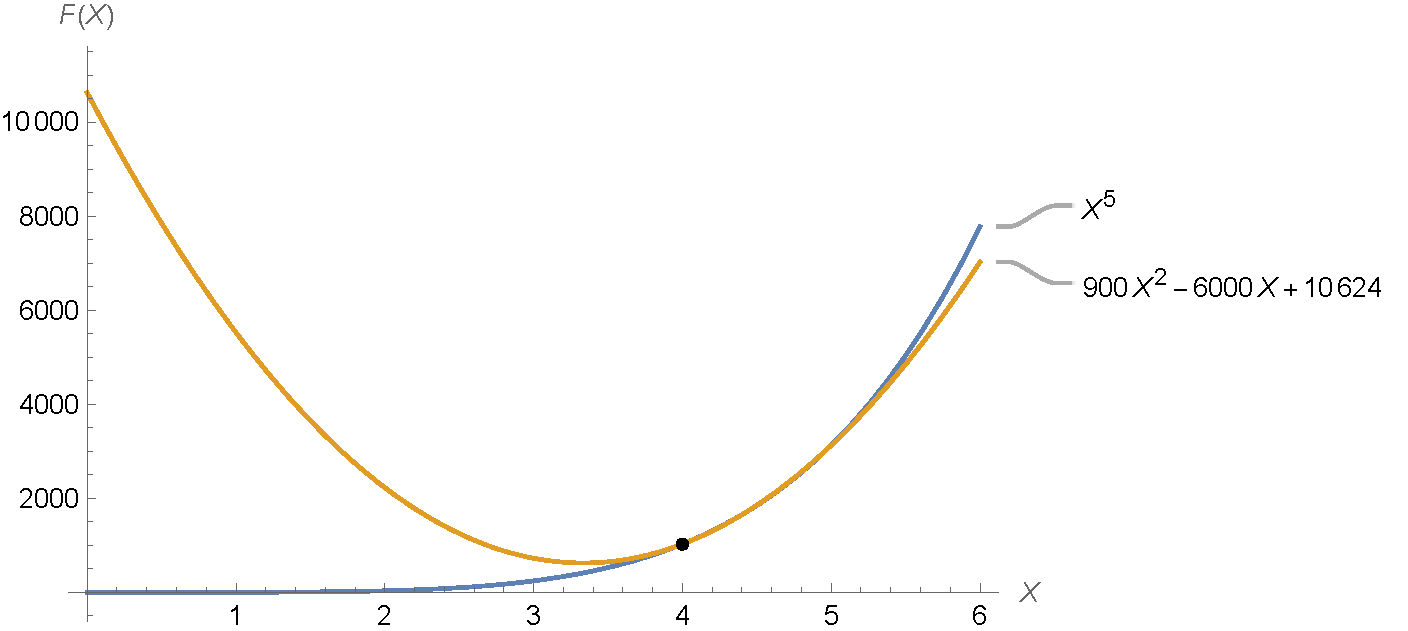
\includegraphics[width=1\textwidth]{sections/images/03_plots_polynomial_p2_n4_with_fifth}
    ~\caption{Approximation of fifth power $X^5$ by $P(2, X, 4)$.
    Convergence interval is $4.0 \leq X \leq 5.1$ with a percentage error $E < 1\%$.
    }\label{fig:03_plots_polynomial_p2_n4_with_fifth}
\end{figure}
Another remarkable observation is
One more interesting observation arises by increasing the value of $N$ in $P(m, X, N)$ while keeping $m$ fixed.
As $N$ increases, the length of the convergence interval with the odd-power $X^{2m+1}$ also increases.
For instance,
\begin{itemize}
    \item For $P(2, X, 4)$ and $X^5$, the convergence interval with a percentage error less than $1\%$ is $4.0 \leq X \leq 5.1$, with a length $L=1.1$
    \item For $P(2, X, 20)$ and $X^5$, the convergence interval with a percentage error less than $1\%$ is $18.7 \leq X \leq 22.9$, with a length $L=4.2$
    \item For $P(2, X, 120)$ and $X^5$, the convergence interval with a percentage error less than $1\%$ is $110.0 \leq X \leq 134.7$, with a length $L=24.7$
\end{itemize}


\subsection{Two-sided Faulhaber's formulas}
\label{subsec:two-sided-faulhaber's-formulas}


\subsection{Derivatives}
\label{subsec:derivatives}




    \section{Future research}\label{sec:future-research}
    Several promising directions emerge from the findings of this manuscript:

\begin{itemize}
    \item \textbf{Integration into mathematical literature.}
    The identities presented in this work do not appear in standard mathematical references,
    despite their elementary nature and apparent classical flavor.
    Notably, related sequences are absent from major repositories such as the OEIS\@.
    Future work should investigate the originality of these results and aim to contextualize
    them within the broader mathematical framework.

    \item \textbf{Extension of approximation methods.}
    The approximation technique developed in~\cite{kolosov2025efficient} is generalizable
    to a broader class of polynomials.
    In particular, by leveraging the symmetry property~\eqref{prop:Tm-symmetry},
    one could explore alternative summation domains for the polynomials $P(m, X, N)$.

    \item \textbf{Combinatorial interpretation of $T_m(n,k)$.}
    The polynomial family $T_m(n,k)$, introduced in~\eqref{def:bivariate-sum-Tm},
    currently lacks a clear combinatorial interpretation.
    Understanding its structural or enumerative significance would deepen insight into
    the algebraic identities presented.

    \item \textbf{Connection with finite differences and derivatives.}
    The binomial form of the odd power identity~\eqref{prop:binomial-form} offers a mechanism
    to express both finite differences and classical derivatives of odd powers in terms
    of the coefficients $\coeffA{m}{r}$.

    \item \textbf{$q$-derivative representation.}
    The general identity~\eqref{theorem:odd-power-identity} also suggests a natural
    expression for $q$-derivatives via the coefficients $\coeffA{m}{r}$,
    potentially leading to a generalized notion of differentiation through limiting procedures.
\end{itemize}



    \section{Conclusions}\label{sec:conclusions}
    This work began with a seemingly elementary interpolation problem and evolved into a broader
investigation of polynomial identities involving odd powers.
Starting from the finite differences of the cubic function, we uncovered a nontrivial identity
that served as a base case for a family of structured decompositions of $n^{2m+1}$.
These identities were expressed in terms of symmetric bivariate sums with recursively defined coefficients.
By employing systems of linear equations and a generating function approach,
we derived both closed-form expressions and recurrence relations for these identities.
The results were further extended to include binomial forms of odd power identities
and formulas for the sums of odd powers.
Computational experiments in \textit{Mathematica} confirmed all theoretical claims and provided
a toolkit for further exploration.
These findings not only contribute novel results to the theory of polynomial identities but also
open pathways to related domains, such as approximation theory and calculus.



    \section*{Acknowledgements}
    The author is grateful to Albert Tkaczyk for pointing out the idea of the general form of odd power identity,
and for providing examples of how to build and solve systems of linear equations to evaluate
the coefficients $\coeffA{m}{r}$.
The author is grateful to Dr. Max Alekseyev (George Washington University) for providing a valuable contribution
of recurrence relation~\eqref{prop:coefficients_a}.
The author is grateful to Markus Scheuer for his elegant and beautiful proof
of the lemma~\eqref{lem:altering-binomial-identity}, see~\cite{scheuer2023mathstackexchange}.
Finally, the author is grateful to OEIS editors for their valuable work during the contribution of sequences
related to this manuscript.


    \bibliographystyle{unsrt}
    \bibliography{unexpected-polynomial-identities-classical-interpolation}

    \noindent \textbf{Version:} \texttt{Local-0.1.0}
\\[1em]
\noindent \textbf{License:} This work is licensed under a
\href{https://creativecommons.org/licenses/by/4.0/}
{\texttt{Creative Commons Attribution 4.0 International License (CC BY 4.0)}}.
\\[1em]
\noindent \textbf{Sources}:
\href{https://github.com/kolosovpetro/unexpected-polynomial-identities-classical-interpolation}
{\texttt{github.com/kolosovpetro/surprising-polynomial-identities}}


    \clearpage


    \section*{Application 1: Mathematica programs}
    We support our theoretical findings with Wolfram~Mathematica programs that verify the main results of this manuscript.
All source code and computational notebooks are available in the
\href{https://github.com/kolosovpetro/surprising-polynomial-identities-classical-interpolation}
{\texttt{GitHub repository}}.
The repository includes the following files:
\begin{itemize}
    \item \texttt{surprising-polynomial-identities-classical-interpolation.m} --- the package file where
    all Mathematica functions are defined.
    Load it into your session using \texttt{filename.m} or by evaluating the file with \texttt{Shift+Enter}.
    \item \texttt{surprising-polynomial-identities-classical-interpolation.nb} --- a working notebook that demonstrates
    the usage of these functions to validate the manuscript’s results.
\end{itemize}

Below we list the Mathematica functions with their corresponding mathematical statements:
\begin{center}
    \renewcommand{\arraystretch}{1.4}
    \begin{tabular}{ll}
        \toprule
        \textbf{Mathematica function}                 & \textbf{Validates}                                            \\
        \midrule
        \texttt{OddPowerIdentity[n, m]}               & Theorem~\ref{theorem:odd-power-identity}                      \\
        \texttt{OddPowerIdentitySimplified[n, m]}     & Theorem~\ref{theorem:odd-power-identity} (in simplified form) \\
        \texttt{BivariateSumT[m, n, k]}               & Definition~\ref{def:bivariate-sum-Tm}                         \\
        \texttt{RecurrenceForT[m, n, k]}              & Proposition~\ref{prop:Tm-recurrence}                          \\
        \texttt{TableFormBivariateSumT[m, rows]}      & Tabular view of $T_m(n,k)$                                    \\
        \texttt{TableFormRecurrenceForT[m, rows]}     & Tabular view of the recurrence                                \\
        \texttt{OddPowerDecomposition[n, m]}          & Proposition~\ref{prop:odd-power-decomposition}                \\
        \texttt{OddPowerDecompositionMMinus1[n, m]}   & Corollary~\ref{cor:odd-power-decomposition-m-1}               \\
        \texttt{OddPowerBinomialForm[m, n, a]}        & Proposition~\ref{prop:odd-power-binomial}                     \\
        \texttt{OddPowerBinomialFormShifted[m, n, a]} & Corollary~\ref{prop:odd-power-binomial-shifted}               \\
        \bottomrule
    \end{tabular}
\end{center}
To test and experiment with these identities computationally, load the package and call any of the
functions listed above with appropriate parameters.

\textbf{Examples of Mathematica Functions}.
This subsection provides sample evaluations of the Mathematica functions
developed to validate the main results presented in the manuscript.
All computations were performed using the package \\
\texttt{surprising-polynomial-identities-classical-interpolation.m}.

\paragraph{Coefficients \texorpdfstring{$\coeffA{m}{r}$}{A(m,r)} table}
\begin{verbatim}
PrintTriangleA[5]
\end{verbatim}
\begin{align*}
    \begin{array}{l}
        \{1\} \\
        \{1,\ 6\} \\
        \{1,\ 0,\ 30\} \\
        \{1,\ -14,\ 0,\ 140\} \\
        \{1,\ -120,\ 0,\ 0,\ 630\} \\
        \{1,\ -1386,\ 660,\ 0,\ 0,\ 2772\}
    \end{array}
\end{align*}

\paragraph{Odd Power Identity}
\begin{verbatim}
OddPowerIdentity[n, 2]
\end{verbatim}
\begin{align*}
    n + n(1 + n)(-1 + n - n^2 + n^3)
\end{align*}
\begin{verbatim}
OddPowerIdentitySimplified[n, 4]
\end{verbatim}
\begin{align*}
    n^9
\end{align*}

\paragraph{Recurrence and Definition of \texorpdfstring{$T_m(n,k)$}{Tm(n,k)}}
\begin{verbatim}
RecurrenceForT[10, 3, 2]
BivariateSumT[10, 3, 2]
\end{verbatim}
\begin{align*}
    T_{10}(3,2) = 5230176601 \quad \text{(both via recurrence and explicit form)}
\end{align*}
\begin{verbatim}
Expand[BivariateSumT[2, n, k]]
\end{verbatim}
\begin{align*}
    1 + 30k^4 - 60k^3 n + 30k^2 n^2
\end{align*}
\begin{verbatim}
BivariateSumT[2, n, k]
\end{verbatim}
\begin{align*}
    1 + 30k^2(n-k)^2
\end{align*}

\paragraph{Tables of \texorpdfstring{$T_m$}{Tm}}
\begin{verbatim}
TableFormRecurrenceForT[3, 5]
TableFormBivariateSumT[3, 5]
\end{verbatim}
\begin{align*}
    \begin{array}{l}
        \{1\} \\
        \{1,\ 1\} \\
        \{1,\ 127,\ 1\} \\
        \{1,\ 1093,\ 1093,\ 1\} \\
        \{1,\ 3739,\ 8905,\ 3739,\ 1\} \\
        \{1,\ 8905,\ 30157,\ 30157,\ 8905,\ 1\}
    \end{array}
\end{align*}

\paragraph{Odd Power Decomposition}
\begin{verbatim}
OddPowerDecomposition[n, 5]
\end{verbatim}
\begin{align*}
    n^{11}
\end{align*}
\begin{verbatim}
OddPowerDecompositionMMinus1[n, 6]
\end{verbatim}
\begin{align*}
    n^{11}
\end{align*}

\paragraph{Binomial Form and Shifted Version}
\begin{verbatim}
OddPowerBinomialForm[2, 15, 5]
5^5
\end{verbatim}
\begin{align*}
    3125
\end{align*}
\begin{verbatim}
OddPowerBinomialForm[2, n, 3]
Simplify[OddPowerBinomialForm[2, n, 3]]
\end{verbatim}
\begin{align*}
    -7776 + 6480n - 2160n^2 + 360n^3 - 30n^4 + n^5 = (-6 + n)^5
\end{align*}
\begin{verbatim}
OddPowerBinomialForm[3, 16, 4]
8^7
\end{verbatim}
\begin{align*}
    2097152
\end{align*}
\begin{verbatim}
Simplify[OddPowerBinomialFormShifted[2, n, 2]]
\end{verbatim}
\begin{align*}
(-4 + n)
    ^5
\end{align*}

These examples confirm the correctness of main results of this manuscript.



    \clearpage


    \section*{Application 2: Examples of coefficients A}
    Consider the definition~\eqref{eq:definition_coefficient_a} of the coefficients $\coeffA{m}{r}$, it can be written as
\begin{equation*}
    \coeffA{m}{r} =
    \begin{cases}
    (2r+1)
        \binom{2r}{r}, & \text{if } r=m; \\
        \sum_{d \geq 2r+1}^{m} \coeffA{m}{d} \underbrace{(2r+1) \binom{2r}{r} \binom{d}{2r+1} \frac{(-1)^{d-1}}{d-r} \bernoulli{2d-2r}}_{T(d,r)}, & \text{if } 0 \leq r<m; \\
        0, & \text{if } r<0 \text{ or } r>m,
    \end{cases}
\end{equation*}
Therefore, let be a definition of the real coefficient $T(d,r)$
\begin{definition}
    Real coefficient $T(d,r)$
    \begin{equation*}
        T(d,r) = (2r+1) \binom{2r}{r} \binom{d}{2r+1} \frac{(-1)^{d-1}}{d-r} \bernoulli{2d-2r}
    \end{equation*}
\end{definition}
\begin{example}
    Let be $m=2$ so first we get $\coeffA{2}{2}$
    \begin{equation*}
        \coeffA{2}{2} = 5\binom{4}{2}=30
    \end{equation*}
    Then $\coeffA{2}{1} = 0$ because $\coeffA{m}{d}$ is zero in the range $m/2 \leq d < m$ means that zero for $d$
    in $1 \leq d < 2$.
    Finally, the coefficient $\coeffA{2}{0}$ is
    \begin{equation*}
        \begin{split}
            \coeffA{2}{0}
            = \sum_{d \geq 1}^{2} \coeffA{2}{d} \cdot T(d, 0)
            &= \coeffA{2}{1} \cdot T(1, 0) + \coeffA{2}{2} \cdot T(2, 0) \\
            &= 30 \cdot \frac{1}{30} = 1
        \end{split}
    \end{equation*}
\end{example}
\begin{example}
    Let be $m=3$ so that first we get $\coeffA{3}{3}$
    \begin{equation*}
        \coeffA{3}{3} = 7 \binom{6}{3}= 140
    \end{equation*}
    Then $\coeffA{3}{2} = 0$ because $\coeffA{m}{d}$ is zero in the range $m/2 \leq d < m$ means that zero for $d$
    in $2 \leq d < 3$.
    The $\coeffA{3}{1}$ coefficient is non-zero and calculated as
    \begin{equation*}
        \begin{split}
            \coeffA{3}{1} = \sum_{d \geq 3}^{3} \coeffA{3}{d} \cdot T(d,1) = \coeffA{3}{3} \cdot T(3,1)
            = 140 \cdot \left( -\frac{1}{10} \right) = -14
        \end{split}
    \end{equation*}
    Finally, the coefficient $\coeffA{3}{0}$ is
    \begin{equation*}
        \begin{split}
            \coeffA{3}{0}= \sum_{d \geq 1}^{3} \coeffA{3}{d} \cdot T(d,0)
            &= \coeffA{3}{1} \cdot T(1,0) + \coeffA{3}{2} \cdot T(2,0) + \coeffA{3}{3} \cdot T(3,0) \\
            &= -14 \cdot \frac{1}{6} + 140 \cdot \frac{1}{42} = 1
        \end{split}
    \end{equation*}
\end{example}
\begin{example}
    Let be $m=4$ so that first we get $\coeffA{4}{4}$
    \begin{equation*}
        \coeffA{4}{4} = 9 \binom{8}{4}= 630
    \end{equation*}
    Then $\coeffA{4}{3} = 0$ and $\coeffA{4}{2} = 0$
    because $\coeffA{m}{d}$ is zero in the range $m/2 \leq d < m$ means that zero for $d$ in $2 \leq d < 4$.
    The value of the coefficient $\coeffA{4}{1}$ is non-zero and calculated as
    \begin{equation*}
        \begin{split}
            \coeffA{4}{1}
            = \sum_{d \geq 3}^{4} \coeffA{4}{d} \cdot T(d,1)
            = \coeffA{4}{3} \cdot T(3,1) + \coeffA{4}{4} \cdot T(4,1)
            = 630 \cdot \left( -\frac{4}{21} \right)
            = -120
        \end{split}
    \end{equation*}
    Finally, the coefficient $\coeffA{4}{0}$ is
    \begin{equation*}
        \begin{split}
            \coeffA{4}{0}
            = \sum_{d \geq 1}^{4} \coeffA{4}{d} \cdot T(d, 0)
            = \coeffA{4}{1} \cdot T(1, 0) + \coeffA{4}{4} \cdot T(4, 0)
            = -120 \cdot \frac{1}{6} + 630 \cdot \frac{1}{30} = 1
        \end{split}
    \end{equation*}
\end{example}
\begin{example}
    Let be $m=5$ so that first we get $\coeffA{5}{5}$
    \begin{equation*}
        \coeffA{5}{5} = 11 \binom{10}{5}= 2772
    \end{equation*}
    Then $\coeffA{5}{4} = 0$ and $\coeffA{5}{3} = 0$
    because $\coeffA{m}{d}$ is zero in the range $m/2 \leq d < m$ means that zero for $d$ in $3 \leq d < 5$.
    The value of the coefficient $\coeffA{5}{2}$ is non-zero and calculated as
    \begin{equation*}
        \begin{split}
            \coeffA{5}{2}
            = \sum_{d \geq 5}^{5} \coeffA{5}{d} \cdot T(d,2) = \coeffA{5}{5} \cdot T(5,2) = 2772 \cdot \frac{5}{21} = 660
        \end{split}
    \end{equation*}
    The value of the coefficient $\coeffA{5}{1}$ is non-zero and calculated as
    \begin{equation*}
        \begin{split}
            \coeffA{5}{1}
            &= \sum_{d \geq 3}^{5} \coeffA{5}{d} \cdot T(d,1)
            = \coeffA{5}{3} \cdot T(3,1) + \coeffA{5}{4} \cdot T(4,1) + \coeffA{5}{5} \cdot T(5,1) \\
            &= 2772 \cdot \left( - \frac{1}{2} \right) = -1386
        \end{split}
    \end{equation*}
    Finally, the coefficient $\coeffA{5}{0}$ is
    \begin{equation*}
        \begin{split}
            \coeffA{5}{0}
            &= \sum_{d \geq 1}^{5} \coeffA{5}{d} \cdot T(d, 0)
            = \coeffA{5}{1} \cdot T(1, 0) + \coeffA{5}{2} \cdot T(2, 0) + \coeffA{5}{5} \cdot T(5, 0) \\
            &= -1386 \cdot \frac{1}{6} + 660 \cdot \frac{1}{30} + 2772 \cdot \frac{5}{66} = 1
        \end{split}
    \end{equation*}
\end{example}


    \clearpage


    \section*{Application 3: Systems of linear equations examples}
    \begin{example}
    Let be $m=3$ so that we have the following relation defined by~\eqref{theorem:odd-power-identity}
    \begin{equation*}
        \coeffA{m}{0} n
        + \coeffA{m}{1} \left[ \frac{1}{6} (-n + n^3) \right]
        + \coeffA{m}{2} \left[ \frac{1}{30} (-n + n^5) \right]
        + \coeffA{m}{3} \left[ \frac{1}{420} (-10 n + 7 n^3 + 3 n^7) \right] - n^7 = 0
    \end{equation*}
    Multiplying by $420$ right-hand side and left-hand side, we get
    \begin{equation*}
        420 \coeffA{3}{0} n + 70 \coeffA{2}{1} (-n + n^3) + 14 \coeffA{2}{2} (-n + n^5) + \coeffA{3}{3} (-10 n + 7 n^3 + 3 n^7) - 420n^7 = 0
    \end{equation*}
    Opening brackets and rearranging the terms gives
    \begin{equation*}
        \begin{split}
            420 \coeffA{3}{0} n
            &- 70 \coeffA{3}{1} + 70 \coeffA{3}{1} n^3 - 14 \coeffA{3}{2} n + 14 \coeffA{3}{2} n^5 \\
            &- 10 \coeffA{3}{3} n + 7 \coeffA{3}{3} n^3 + 3 \coeffA{3}{3} n^7 - 420n^7 = 0
        \end{split}
    \end{equation*}
    Combining the common terms yields
    \begin{equation*}
        \begin{split}
            &n (420 \coeffA{3}{0} - 70 \coeffA{3}{1} - 14 \coeffA{3}{2} - 10 \coeffA{3}{3}) \\
            &+ n^3 (70 \coeffA{3}{1} + 7 \coeffA{3}{3})
            + n^5 14 \coeffA{3}{2}
            + n^7 (3 \coeffA{3}{3} - 420)
            = 0
        \end{split}
    \end{equation*}
    Therefore, the system of linear equations follows
    \begin{equation*}
        \begin{cases}
            420 \coeffA{3}{0} - 70 \coeffA{3}{1} - 14 \coeffA{3}{2} - 10 \coeffA{3}{3} = 0 \\
            70 \coeffA{3}{1} + 7 \coeffA{3}{3} = 0 \\
            \coeffA{3}{2} - 30 = 0 \\
            3 \coeffA{3}{3} - 420 = 0
        \end{cases}
    \end{equation*}
    Solving it, we get
    \begin{equation*}
        \begin{cases}
            \coeffA{3}{3} = 140 \\
            \coeffA{3}{2} = 0 \\
            \coeffA{3}{1} = -\frac{7}{70} \coeffA{3}{3} = -14 \\
            \coeffA{3}{0} = \frac{(70 \coeffA{3}{1} + 10 \coeffA{3}{3})}{420} = 1
        \end{cases}
    \end{equation*}
    So that odd-power identity~\eqref{theorem:odd-power-identity} holds
    \begin{equation*}
        n^7 = \sum_{k=1}^{n} 140 k^3 (n-k)^3 - 14k(n-k) + 1
    \end{equation*}
    It is also clearly seen
    why the above identity is true evaluating the terms $140 k^3 (n-k)^3 - 14k(n-k) + 1$ over $0 \leq k \leq n$ as
    the OEIS sequence \href{https://oeis.org/A300785}{\textit{A300785}}
    ~\cite{oeis_numerical_triangle_row_sums_give_seventh_powers} shows
    \begin{table}[H]
    \setlength\extrarowheight{-6pt}
    \begin{tabular}{c|cccccccc}
        $n/k$ & 0 & 1     & 2      & 3      & 4      & 5      & 6     & 7 \\
        \hline
        0     & 1 &       &        &        &        &        &       &   \\
        1     & 1 & 1     &        &        &        &        &       &   \\
        2     & 1 & 127   & 1      &        &        &        &       &   \\
        3     & 1 & 1093  & 1093   & 1      &        &        &       &   \\
        4     & 1 & 3739  & 8905   & 3739   & 1      &        &       &   \\
        5     & 1 & 8905  & 30157  & 30157  & 8905   & 1      &       &   \\
        6     & 1 & 17431 & 71569  & 101935 & 71569  & 17431  & 1     &   \\
        7     & 1 & 30157 & 139861 & 241753 & 241753 & 139861 & 30157 & 1
    \end{tabular}
    \caption{Values of $140 k^3 (n-k)^3 - 14k(n-k) + 1$.
    See the OEIS entry \href{https://oeis.org/A300785}{\texttt{A300785}}
    ~\cite{oeis_numerical_triangle_row_sums_give_seventh_powers}.}
    \label{tab:row-sums-gives-seventh-power}
\end{table}

\end{example}

\begin{example}
    Let be $m=4$ so that we have the following relation defined by~\eqref{theorem:odd-power-identity}
    \begin{equation*}
        \begin{split}
            \coeffA{m}{0} n
            &+ \coeffA{m}{1} \left[ \frac{1}{6} (-n + n^3) \right]
            + \coeffA{m}{2} \left[ \frac{1}{30} (-n + n^5) \right] \\
            &+ \coeffA{m}{3} \left[ \frac{1}{420} (-10 n + 7 n^3 + 3 n^7) \right] \\
            &+ \coeffA{m}{4} \left[ \frac{1}{630} (-21 n + 20 n^3 + n^9) \right] - n^9 = 0
        \end{split}
    \end{equation*}
    Multiplying by $630$ right-hand side and left-hand side, we get
    \begin{equation*}
        \begin{split}
            630 \coeffA{4}{0} n
            &+ 105 \coeffA{4}{1} (-n + n^3) + 21 \coeffA{4}{2} (-n + n^5) \\
            &+ \frac{3}{2} \coeffA{4}{3} (-10 n + 7 n^3 + 3 n^7) \\
            &+ \coeffA{4}{4} (-21 n + 20 n^3 + n^9) - 630 n^9 = 0
        \end{split}
    \end{equation*}
    Opening brackets and rearranging the terms gives
    \begin{equation*}
        \begin{split}
            630 \coeffA{4}{0} n
            &- 105 \coeffA{4}{1} n + 105 \coeffA{4}{1} n ^3 - 21 \coeffA{4}{2} n + 21 \coeffA{4}{2} n^5 \\
            &- \frac{3}{2} \coeffA{4}{3} \cdot 10n + \frac{3}{2} \coeffA{4}{3} \cdot 7n^3 + \frac{3}{2} \coeffA{4}{3} \cdot 3n^7 \\
            &-21 \coeffA{4}{4} n + 20 \coeffA{4}{4} n^3 + \coeffA{4}{4} n ^9 - 630 n^9 = 0
        \end{split}
    \end{equation*}
    Combining the common terms yields
    \begin{equation*}
        \begin{split}
            &n (630 \coeffA{4}{0} - 105 \coeffA{4}{1} - 21 \coeffA{4}{2} - 15 \coeffA{4}{3} - 21 \coeffA{4}{4})  \\
            &+ n^3 \left( 105 \coeffA{4}{1} + \frac{21}{2} \coeffA{4}{3} + 20 \coeffA{4}{4} \right) + n^5 (21 \coeffA{4}{2}) \\
            &+ n^7 \left( \frac{9}{2} \coeffA{4}{3} \right) + n^9 (\coeffA{4}{4} - 630) = 0
        \end{split}
    \end{equation*}
    Therefore, the system of linear equations follows
    \begin{equation*}
        \begin{cases}
            630 \coeffA{4}{0} - 105 \coeffA{4}{1} - 21 \coeffA{4}{2} - 15 \coeffA{4}{3} - 21 \coeffA{4}{4} = 0 \\
            105 \coeffA{4}{1} + \frac{21}{2} \coeffA{4}{3} + 20 \coeffA{4}{4} = 0 \\
            \coeffA{4}{2} = 0 \\
            \coeffA{4}{3} = 0 \\
            \coeffA{4}{4} - 630 = 0
        \end{cases}
    \end{equation*}
    Solving it, we get
    \begin{equation*}
        \begin{cases}
            \coeffA{4}{4} = 630 \\
            \coeffA{4}{3} = 0 \\
            \coeffA{4}{2} = 0 \\
            \coeffA{4}{1} = - \frac{20}{105} \coeffA{4}{4} = -120 \\
            \coeffA{4}{0} = \frac{105 \coeffA{4}{1} + 21 \coeffA{4}{4}}{630} = 1
        \end{cases}
    \end{equation*}
    So that odd-power identity~\eqref{theorem:odd-power-identity} holds
    \begin{equation*}
        n^9 = \sum_{k=1}^{n} 630 k^4(n-k)^4 - 120k(n-k) + 1
    \end{equation*}
\end{example}


    \clearpage


    \section*{Application 4: Related OEIS sequences}
    \begin{center}
    \renewcommand{\arraystretch}{1.3}
    \begin{tabular}{lll}
        \toprule
        \textbf{OEIS ID} & \textbf{Description}                                                 & \textbf{Citation}                                                  \\
        \midrule
        \texttt{A287326} & Numerical triangle, row sums give third power                        & ~\cite{oeis_numerical_triangle_row_sums_give_cubes}                \\
        \texttt{A300656} & Numerical triangle, row sums give fifth power                        & ~\cite{oeis_numerical_triangle_row_sums_give_fifth_powers}         \\
        \texttt{A300785} & Numerical triangle, row sums give seventh power                      & ~\cite{oeis_numerical_triangle_row_sums_give_seventh_powers}       \\
        \texttt{A302971} & Numerators of the coefficient $\coeffA{m}{r}$                        & ~\cite{oeis_numerators_of_the_coefficient_a_m_r}                   \\
        \texttt{A304042} & Denominators of the coefficient $\coeffA{m}{r}$                      & ~\cite{oeis_denominators_of_the_coefficient_a_m_r}                 \\
        \texttt{A320047} & Coefficients $U(m, l, k)$ for $m = 1$ defined by polynomial identity & ~\cite{oeis_coefficients_u_m_l_k_defined_by_polynomial_identity_1} \\
        \texttt{A316349} & Coefficients $U(m, l, k)$ for $m = 2$ defined by polynomial identity & ~\cite{oeis_coefficients_u_m_l_k_defined_by_polynomial_identity_2} \\
        \texttt{A316387} & Coefficients $U(m, l, k)$ for $m = 3$ defined by polynomial identity & ~\cite{oeis_coefficients_u_m_l_k_defined_by_polynomial_identity_3} \\
        \bottomrule
    \end{tabular}
\end{center}


\end{document}
